%%%%%%%%%%%%%%%%%%%%%%%%%%%%%%%%%%%%%%%%%
% Jacobs Landscape Poster
% LaTeX Template
% Version 1.1 (14/06/14)
%
% Created by:
% Computational Physics and Biophysics Group, Jacobs University
% https://teamwork.jacobs-university.de:8443/confluence/display/CoPandBiG/LaTeX+Poster
% 
% Further modified by:
% Nathaniel Johnston (nathaniel@njohnston.ca)
%
% This template has been downloaded from:
% http://www.LaTeXTemplates.com
%
% License:
% CC BY-NC-SA 3.0 (http://creativecommons.org/licenses/by-nc-sa/3.0/)
%
%%%%%%%%%%%%%%%%%%%%%%%%%%%%%%%%%%%%%%%%%

%----------------------------------------------------------------------------------------
%	PACKAGES AND OTHER DOCUMENT CONFIGURATIONS
%----------------------------------------------------------------------------------------

\documentclass[final]{beamer}

\usepackage[scale=1.24]{beamerposter} % Use the beamerposter package for laying out the poster

\usetheme{confposter} % Use the confposter theme supplied with this template

\setbeamercolor{block title}{fg=ngreen,bg=white} % Colors of the block titles
\setbeamercolor{block body}{fg=black,bg=white} % Colors of the body of blocks
\setbeamercolor{block alerted title}{fg=white,bg=dblue!70} % Colors of the highlighted block titles
\setbeamercolor{block alerted body}{fg=black,bg=dblue!10} % Colors of the body of highlighted blocks
% Many more colors are available for use in beamerthemeconfposter.sty

%-----------------------------------------------------------
% Define the column widths and overall poster size
% To set effective sepwid, onecolwid and twocolwid values, first choose how many columns you want and how much separation you want between columns
% In this template, the separation width chosen is 0.024 of the paper width and a 4-column layout
% onecolwid should therefore be (1-(# of columns+1)*sepwid)/# of columns e.g. (1-(4+1)*0.024)/4 = 0.22
% Set twocolwid to be (2*onecolwid)+sepwid = 0.464
% Set threecolwid to be (3*onecolwid)+2*sepwid = 0.708

\newlength{\sepwid}
\newlength{\onecolwid}
\newlength{\twocolwid}
\newlength{\threecolwid}
\setlength{\paperwidth}{48in} % A0 width: 46.8in
\setlength{\paperheight}{36in} % A0 height: 33.1in
\setlength{\sepwid}{0.024\paperwidth} % Separation width (white space) between columns
\setlength{\onecolwid}{0.22\paperwidth} % Width of one column
\setlength{\twocolwid}{0.464\paperwidth} % Width of two columns
\setlength{\threecolwid}{0.708\paperwidth} % Width of three columns
\setlength{\topmargin}{-0.5in} % Reduce the top margin size
%-----------------------------------------------------------

\usepackage{graphicx}  % Required for including images

\usepackage{booktabs} % Top and bottom rules for tables

%----------------------------------------------------------------------------------------
%	TITLE SECTION 
%----------------------------------------------------------------------------------------

\title{SOFTWARE ENGINEERING PROCESSES--CALCULATOR} %CPoster title

\author{Jingya Pan} % Author(s)

\institute{Gina Cody School of Engineering and Computer Science,Concordia University} % Institution(s)

%----------------------------------------------------------------------------------------

\begin{document}

\addtobeamertemplate{block end}{}{\vspace*{2ex}} % White space under blocks
\addtobeamertemplate{block alerted end}{}{\vspace*{2ex}} % White space under highlighted (alert) blocks

\setlength{\belowcaptionskip}{2ex} % White space under figures
\setlength\belowdisplayshortskip{2ex} % White space under equations

\begin{frame}[t] % The whole poster is enclosed in one beamer frame

\begin{columns}[t] % The whole poster consists of three major columns, the second of which is split into two columns twice - the [t] option aligns each column's content to the top

\begin{column}{\sepwid}\end{column} % Empty spacer column

\begin{column}{\onecolwid} % The first column

%----------------------------------------------------------------------------------------
%	Introduction
%----------------------------------------------------------------------------------------

\begin{alertblock}{Introduction}

F5: $\Gamma \left( x \right)$ which is named as gamma function, is a commonly used extension of the factorial function to complex numbers\\
\begin{itemize}
\item For the gamma function, 0 and all the negative integers are not defined.
\item  When  for any positive integer a, then the gamma function is related to the factorial function  $\Gamma(a) = (a-1)!$ \\
\item For complex numbers with a positive real part, then the gamma function is defined as ${\displaystyle \Gamma (a)=\int _{0}^{\infty }x^{a-1}e^{-x}\,dx.}$ 
\item The previous definition can be extended to the whole complex number domain except negative integer by using  analytic continuation.
\end{itemize}

\end{alertblock}

%----------------------------------------------------------------------------------------
%	Requirements
%----------------------------------------------------------------------------------------

\begin{block}{Requirements}

\begin{enumerate}
\item \textbf{R1}:When the user entered the parameter a, the calculating system shall verify the validation of the parameter. If it is not valid, show up the error message and give the tip and instruct the user to enter the value with correct format.
\setlength{\itemsep}{6pt}
\item \textbf{R2}:When the parameter a for the gamma function is received,the calculating system shall process the gamma function with the received parameter a within  2 or 3 seconds.
\setlength{\itemsep}{6pt}
\item \textbf{R3}:The result of the calculating system shall be accurate and correct after user giving a valid input.
\setlength{\itemsep}{6pt}
\item \textbf{R4}:The calculating system shall be maintainable.
\end{enumerate}

\end{block}

%------------------------------------------------

\begin{figure}
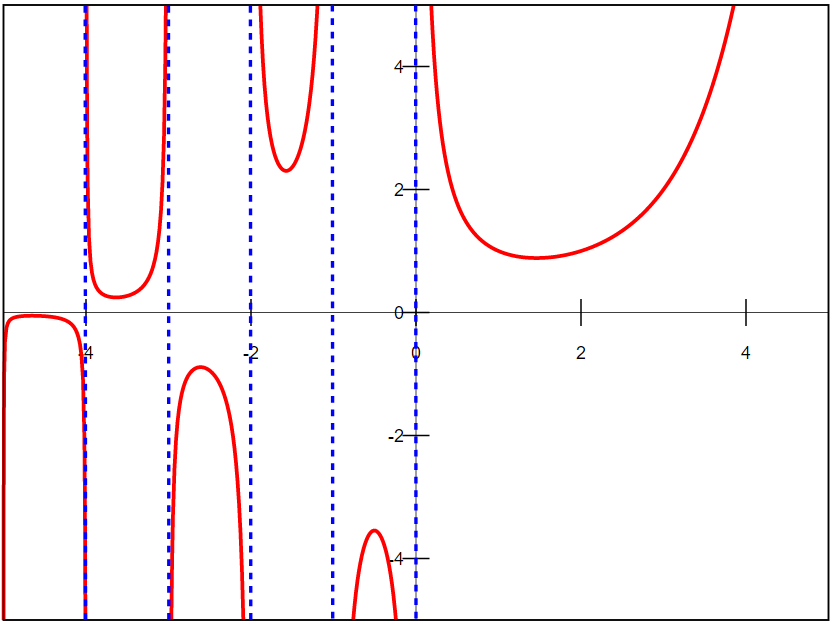
\includegraphics[width=0.7\linewidth]{gamma.png}
\caption{Gamma Function}
\end{figure}

%----------------------------------------------------------------------------------------

\end{column} % End of the first column

\begin{column}{\sepwid}\end{column} % Empty spacer column

\begin{column}{\twocolwid} % Begin a column which is two columns wide (column 2)

\begin{columns}[t,totalwidth=\twocolwid] % Split up the two columns wide column

\begin{column}{\onecolwid}\vspace{-.6in} % The first column within column 2 (column 2.1)

%----------------------------------------------------------------------------------------
%	Approach
%----------------------------------------------------------------------------------------

\begin{block}{Approach}

\begin{itemize}
\setlength{\itemsep}{20pt}
\item \textbf{Algorithm}:There are 2 methods to implement gamma function, namely Lanczos approximation and Stirling's approximation. Comparing output of two methods, Lanczos approximation is more accurate and is used to serve for implementation.
\setlength{\itemsep}{20pt}
\item \textbf{Debugger}:Debugger support in eclipse is used to debug this calculator application. Eclipse IDE support the debug perspective which can be run easily to check the intermediate status of variable.
\setlength{\itemsep}{20pt}
\item \textbf{Quality Check}: The 'Checkstyle' plugin for eclipse is used to review the code specification and ensure that java code follows a standard code style, which saves plenty of time to check the coding standard manually line by line, and it allows us to easily modify the improper format by following the given instruction.

\end{itemize}

\end{block}

%----------------------------------------------------------------------------------------

\end{column} % End of column 2.1

\begin{column}{\onecolwid}\vspace{-.6in} % The second column within column 2 (column 2.2)

%----------------------------------------------------------------------------------------
%	METHODS
%----------------------------------------------------------------------------------------

\begin{block}{Quality Attributes}
\begin{itemize}
\setlength{\itemsep}{20pt}
\item \textbf{Usable}:The calculator application provides a relative easy and clear front look, which will less likely to make user get confused.
\item \textbf{Maintainable}:The calculator application is maintainable because of the separation of  the function modules.Therefore the application will be maintainable and modifiable for the future changes.
\item \textbf{Correct}:The correctness and accuracy is the primary request for the calculator application, since it calculate to 15 decimal place.
\item \textbf{Efficient}:The calculator application is efficient which is achieved by simple and clear process.
\item \textbf{Robust}:The calculator application is robust which is achieved by concerning the extreme cases and dealing with them correspondingly.

\end{itemize}

\end{block}

%----------------------------------------------------------------------------------------

\end{column} % End of column 2.2

\end{columns} % End of the split of column 2 - any content after this will now take up 2 columns width

%----------------------------------------------------------------------------------------
%	IMPORTANT RESULT
%----------------------------------------------------------------------------------------

\begin{alertblock}{Important Result}

The following part includes the graphical user interface as a result of the project and also suggestions I got from my teammates during the reviewing and testing session.
\end{alertblock} 

%----------------------------------------------------------------------------------------

\begin{columns}[t,totalwidth=\twocolwid] % Split up the two columns wide column again

\begin{column}{\onecolwid} % The first column within column 2 (column 2.1)

%----------------------------------------------------------------------------------------
%	Source code review
%----------------------------------------------------------------------------------------

\begin{block}{Source Code Review}

\begin{itemize}
\setlength{\itemsep}{20pt}
\item \textbf{Code distribution}: The main file includes both functional code and configuration code, which makes the code is not properly distributed. Therefore I separate the main file into two files for better understanding.
\setlength{\itemsep}{60pt}
\item \textbf{Duplicate code}: The method size is not that reasonable which makes it not easy to keep manageable. Too many conditions fragments exist, so the refactoring is applied to the specific method.

\end{itemize}

\end{block}

%----------------------------------------------------------------------------------------

\end{column} % End of column 2.1

\begin{column}{\onecolwid} % The second column within column 2 (column 2.2)

%----------------------------------------------------------------------------------------
%	RESULTS
%----------------------------------------------------------------------------------------

\begin{block}{Results}

\begin{figure}
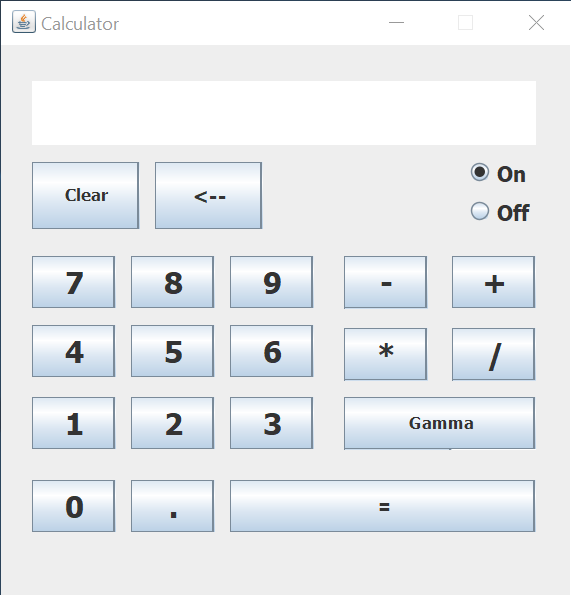
\includegraphics[width=0.7\linewidth]{calculator.png}
\caption{Calculator user interface}
\end{figure}


\end{block}

%----------------------------------------------------------------------------------------

\end{column} % End of column 2.2

\end{columns} % End of the split of column 2

\end{column} % End of the second column

\begin{column}{\sepwid}\end{column} % Empty spacer column

\begin{column}{\onecolwid} % The third column

%----------------------------------------------------------------------------------------
%	Test cases review
%----------------------------------------------------------------------------------------

\begin{block}{Test Cases Review}
The following table is the test result based on gamma function method, according to the comparison between the expected and obtained value, it can tell that the deviation is within the range.
\noindent
\begin{table}
\begin{tabular}{l l l}
\toprule
\textbf{Input } & \textbf{ Expected Value} & \textbf{Obtained Value}\\
\midrule
1 &  1.0 & 0.9999999999999998 \\
-2.4 &  -1.108029947033346058329 & -1.108029947033344 \\
1.5 &  0.8862269254527580136491 & 0.8862269254527586 \\
\bottomrule
\end{tabular}
\caption{Gamma function Testing Result Table}
\end{table}

\end{block}

%----------------------------------------------------------------------------------------
%	CONCLUSION
%----------------------------------------------------------------------------------------

\begin{block}{Conclusion}

Form this calculator application, a process is followed from the very start to collect the background knowledge, and based on that the requirements are analyzed. After the brainstorming about the pseudo code format within the group range, the implementation phase starts, followed by debugging and code standard checking. Finally, from the peer review, I learned a lot and refactored my code accordingly.

\end{block}

%----------------------------------------------------------------------------------------
%	REFERENCES
%----------------------------------------------------------------------------------------

\begin{block}{References}

\begin{itemize}
\setlength{\itemsep}{20pt}
\item \
[Jekyll.math.byuh.edu]Properties of the Gamma function \\
\indent \indent\indent\indent\indent\indent\indent http://www.jekyll.math.byuh.edu/courses/m321/\\handouts/gammaproperties.pdf

\setlength{\itemsep}{20pt}
\item \
[En.wikipedia.org] Gamma function https://en.wikipedia.org/wiki/Gamma function

\end{itemize}
\end{block}

%----------------------------------------------------------------------------------------
%	ACKNOWLEDGEMENTS
%----------------------------------------------------------------------------------------

\setbeamercolor{block title}{fg=red,bg=white} % Change the block title color

\begin{block}{Acknowledgements}
I do appreciate Professor P. Kamthan and my teammates' help and suggestion.
\end{block}

%----------------------------------------------------------------------------------------
%	CONTACT INFORMATION
%----------------------------------------------------------------------------------------

\setbeamercolor{block alerted title}{fg=black,bg=norange} % Change the alert block title colors
\setbeamercolor{block alerted body}{fg=black,bg=white} % Change the alert block body colors

\begin{alertblock}{Contact Information}

\begin{itemize}
\item Github address : https://github.com/panjingya/SOEN6011.git

\end{itemize}

\end{alertblock}

%----------------------------------------------------------------------------------------

\end{column} % End of the third column

\end{columns} % End of all the columns in the poster

\end{frame} % End of the enclosing frame

\end{document}
